\documentclass[11pt,a4paper]{article}
\usepackage[utf8]{inputenc}
\usepackage[T1]{fontenc}
\usepackage[italian]{babel}
\usepackage[sc]{mathpazo}
\linespread{1.06}
\usepackage{amsmath,amssymb,amsthm,mathtools}
\usepackage[margin=2.5cm]{geometry}
\usepackage{booktabs,array,tabularx}
\usepackage[shortlabels]{enumitem}
\usepackage{microtype}
\usepackage[dvipsnames]{xcolor}
\usepackage[colorlinks=true,linkcolor=MidnightBlue,citecolor=MidnightBlue,urlcolor=MidnightBlue]{hyperref}
\usepackage{graphicx}
\usepackage{tikz}
\usetikzlibrary{arrows.meta,decorations.pathmorphing,calc,positioning}
\usepackage[italian,capitalise,nameinlink]{cleveref}
\crefname{figure}{Figura}{Figure}

\theoremstyle{plain}
\newtheorem{theorem}{Teorema}[section]
\newtheorem{lemma}[theorem]{Lemma}
\newtheorem{proposition}[theorem]{Proposizione}
\newtheorem{corollary}[theorem]{Corollario}
\newtheorem{conjecture}[theorem]{Congettura}
\theoremstyle{definition}
\newtheorem{definition}[theorem]{Definizione}
\newtheorem{hypothesis}[theorem]{Ipotesi}
\theoremstyle{remark}
\newtheorem{remark}[theorem]{Osservazione}
\crefname{theorem}{Teorema}{Teoremi}
\crefname{lemma}{Lemma}{Lemmi}
\crefname{proposition}{Proposizione}{Proposizioni}
\crefname{corollary}{Corollario}{Corollari}
\crefname{conjecture}{Congettura}{Congetture}
\crefname{definition}{Definizione}{Definizioni}
\crefname{hypothesis}{Ipotesi}{Ipotesi}
\crefname{remark}{Osservazione}{Osservazioni}
\crefname{section}{Sezione}{Sezioni}
\crefname{appendix}{Appendice}{Appendici}
\crefname{table}{Tabella}{Tabelle}
\crefname{equation}{}{}

\newcommand{\ket}[1]{\lvert #1\rangle}
\newcommand{\bra}[1]{\langle #1\rvert}
\newcommand{\braket}[2]{\langle #1\vert #2\rangle}
\newcommand{\Stab}{\mathrm{Stab}}
\newcommand{\Paulis}{\mathcal P}
\newcommand{\Fb}{\mathbb F}
\newcommand{\C}{\mathbb C}
\newcommand{\Q}{\mathbb Q}
\newcommand{\Z}{\mathbb Z}
\newcommand{\E}{\mathop{\mathbb E}}
\newcommand{\poly}{\mathrm{poly}}
\newcommand{\polylog}{\mathrm{polylog}}
\newcommand{\ChiP}{\chi_{\otimes}}
\newcommand{\Cl}{\mathcal C}
\newcommand{\eps}{\varepsilon}
\newcommand{\Tst}{\ket{T}}
\newcommand{\Hst}{\ket{H}}
\newcommand{\Gram}{\mathsf G}

\title{\textbf{Process tensor random con rumore}\\[4pt]
\large Due modelli esatti: memoria, Markovianizzazione e free probability}
\author{Nota di lavoro\thanks{Bozza preparata con Claude Code. Tutte le formule sono verificate numericamente (Monte Carlo o ricorsioni esatte indipendenti), ma le derivazioni vanno rilette. Gli script sono nella cartella \texttt{scripts/} accanto ai sorgenti.}}
\date{26 novembre 2026}
% ---------------------------------------------------------------
% Cartoon macros (colours match the plots)
\definecolor{cBlue}{HTML}{257DE0}\definecolor{cOrange}{HTML}{F47230}
\definecolor{cAqua}{HTML}{00B894}\definecolor{cViolet}{HTML}{6A4CE2}
\definecolor{cGray}{HTML}{666666}\definecolor{cDark}{HTML}{191919}
\tikzset{
  gate/.style={draw=cBlue, fill=cBlue!10, rounded corners=2pt, font=\small, inner sep=1pt},
  hgate/.style={draw=cViolet, fill=cViolet!10, rounded corners=2pt, font=\small, inner sep=1pt},
  noise/.style={draw=cOrange, fill=cOrange!15, rounded corners=1pt, font=\scriptsize, inner sep=1.5pt},
  ewire/.style={line width=2.4pt, cGray!45},
  swire/.style={thick, cDark},
  lab/.style={font=\footnotesize, text=cDark},
  small/.style={font=\scriptsize, text=cGray},
}
\newcommand{\meter}[2]{%
  \draw[fill=white, rounded corners=1pt] ($#1+(-0.2,-0.15)$) rectangle ($#1+(0.2,0.15)$);
  \draw ($#1+(-0.12,-0.07)$) arc (160:20:0.13);
  \draw[-{Stealth[length=2pt]}] ($#1+(0,-0.09)$) -- ($#1+(0.09,0.09)$);
  \node[font=\scriptsize, above] at ($#1+(0,0.14)$) {#2};}
% ---------------------------------------------------------------

\newcommand{\CartoonModelOne}{%
\begin{figure}[!htbp]
\centering
\begin{tikzpicture}[x=1cm, y=1cm]
  % ----- circuit
  \node[lab, anchor=east] at (-0.55,0) {$\rho_{\rm E}$};
  \draw[ewire] (-0.5,0) -- (7.3,0);
  \node[small, anchor=west] at (7.35,0) {$\mathrm{Tr}_{\rm E}$};
  \foreach \i/\x in {1/0.6, 2/2.9, 3/5.2} {
    \draw[swire] (\x-0.8,1.1) -- (\x-0.32,1.1); \draw[fill=white] (\x-0.8,1.1) circle (1.6pt);
    \node[small, above] at (\x-0.75,1.13) {$i_{\i}$};
    \draw[swire] (\x+0.32,1.1) -- (\x+0.8,1.1); \draw[fill=white] (\x+0.8,1.1) circle (1.6pt);
    \node[small, above] at (\x+0.75,1.13) {$o_{\i}$};
    \node[gate, minimum width=0.62cm, minimum height=1.55cm] at (\x,0.55) {$U_{\i}$};
    \node[noise] at (\x+1.15,0) {$\mathcal N$};
  }
  \node[lab] at (6.6,0.55) {$\cdots$};
  \node[small, align=left, anchor=west] at (-0.6,-0.65) {ambiente E: $L$ qudit, $D=q^L$ (la memoria); Haar globale su S$\otimes$E a ogni passo, rumore $\mathcal N$ su ogni qudit};
  % ----- MPS in time
  \begin{scope}[yshift=-2.3cm]
    \node[lab, anchor=east] at (-0.55,0) {$\Upsilon_n=$};
    \foreach \i/\x in {1/0.6, 2/2.9, 3/5.2} {
      \draw[swire] (\x-0.12,0.15) -- (\x-0.12,0.7); \draw[swire] (\x+0.12,0.15) -- (\x+0.12,0.7);
      \node[small, above] at (\x,0.68) {$i_{\i}\,o_{\i}$};
      \node[circle, draw=cBlue, fill=cBlue!15, minimum size=0.55cm, inner sep=0pt] (T\i) at (\x,0) {};
    }
    \draw[ewire] (-0.4,0) -- (T1); \draw[ewire] (T1) -- (T2); \draw[ewire] (T2) -- (T3); \draw[ewire] (T3) -- (6.4,0);
    \foreach \x in {1.75, 4.05} {\node[noise] at (\x,0) {$\mathcal N$};}
    \node[lab] at (6.6,0) {$\cdots$};
    \node[small, anchor=west] at (7.0,0) {bond $=D$};
    \node[small, anchor=west] at (-0.6,-0.6) {stato di Choi: un RMPS nel tempo, con dimensione fisica $d^2$ (gambe $i_t,o_t$) e bond dimension $D$};
  \end{scope}
\end{tikzpicture}
\caption{Modello 1. In alto: il circuito di collisione con memoria. Le gambe aperte $i_t$ (ingresso) e $o_t$ (uscita) di S sono quelle di Choi, e il rumore $\mathcal N$ agisce sull'ambiente fra un passo e l'altro. In basso: il process tensor $\Upsilon_n$ è un MPS nel tempo il cui legame è l'ambiente; il rumore agisce sui legami.}
\label{fig:cartoon-m1}
\end{figure}}

\newcommand{\CartoonReplica}{%
\begin{figure}[!htbp]
\centering
\begin{tikzpicture}[x=1cm, y=1cm]
  % ----- identity label (box)
  \begin{scope}[shift={(0,0)}]
    \draw[ewire, cBlue!60] (0,0.35) -- (1.4,0.35); \draw[ewire, cBlue!60] (0,-0.35) -- (1.4,-0.35);
    \node[small, anchor=east] at (0,0.35) {1}; \node[small, anchor=east] at (0,-0.35) {2};
    \node[lab] at (0.7,-0.95) {$\square$: ogni replica};
    \node[lab] at (0.7,-1.3) {tracciata da sé};
  \end{scope}
  % ----- swap label (circle)
  \begin{scope}[shift={(4.4,0)}]
    \draw[ewire, cOrange!70] (0,0.35) .. controls (0.7,0.35) and (0.7,-0.35) .. (1.4,-0.35);
    \draw[ewire, cOrange!70] (0,-0.35) .. controls (0.7,-0.35) and (0.7,0.35) .. (1.4,0.35);
    \node[small, anchor=east] at (0,0.35) {1}; \node[small, anchor=east] at (0,-0.35) {2};
    \node[lab] at (0.7,-0.95) {$\circ$: repliche legate};
    \node[lab] at (0.7,-1.3) {(memoria / eco)};
  \end{scope}
  % ----- transitions
  \draw[-{Stealth[length=5pt]}, thick, cDark] (1.8,0.65) to[out=120, in=60, looseness=4] node[above, lab] {$a\simeq1/d^2$} (2.1,0.65);
  \draw[-{Stealth[length=5pt]}, thick, cDark] (4.25,0.65) to[out=120, in=60, looseness=4] node[above, lab] {$u_{\rm eff}\simeq(g_F/q^2)^L$} (4.55,0.65);
  \draw[-{Stealth[length=5pt]}, thick, cOrange] (4.1,-0.1) -- node[below, lab, text=cOrange] {rumore} (2.0,-0.1);
  % ----- level crossing inset
  \begin{scope}[shift={(7.6,-1.2)}]
    \draw[-{Stealth[length=4pt]}, cGray] (0,0) -- (3.0,0) node[right, small] {$L$};
    \draw[-{Stealth[length=4pt]}, cGray] (0,0) -- (0,2.1) node[above, small] {autovalori};
    \draw[thick, cBlue] (0,0.9) -- (2.8,0.9) node[right, small, text=cBlue] {Markov};
    \draw[thick, cOrange] (0,1.9) .. controls (1.0,1.2) and (1.8,0.6) .. (2.8,0.25) node[right, small, text=cOrange] {memoria};
    \draw[dashed, cGray] (1.32,0) -- (1.32,0.9); \node[small, below] at (1.32,0) {$L^*$};
  \end{scope}
\end{tikzpicture}
\caption{Struttura a due repliche, comune ai due modelli. L'ambiente porta un'etichetta: $\square$ (identità) o $\circ$ (scambio delle repliche). Il rumore agisce replica per replica e quindi smorza solo $\circ$. Nel modello 1 il settore di memoria decade come $(g_F/q^2)^L$ e incrocia il settore Markoviano ($a\simeq1/d^2$) in $L^*$: oltre l'incrocio la memoria crolla.}
\label{fig:cartoon-replica}
\end{figure}}

\newcommand{\CartoonModelTwo}{%
\begin{figure}[!htbp]
\centering
\begin{tikzpicture}[x=1cm, y=1cm]
  % ----- circuit A, C, E
  \node[lab, anchor=east] at (-0.3,1.6) {A}; \node[lab, anchor=east] at (-0.3,0.8) {C}; \node[lab, anchor=east] at (-0.3,0) {E};
  \draw[swire] (-0.25,1.6) -- (6.3,1.6); \draw[swire] (-0.25,0.8) -- (6.3,0.8); \draw[ewire] (-0.25,0) -- (6.3,0);
  \foreach \i/\x in {1/0.4, 2/2.4, 3/4.4} {
    \node[gate, minimum width=0.55cm, minimum height=1.15cm] at (\x,1.2) {$U$};
    \node[hgate, minimum width=0.55cm, minimum height=1.15cm] at (\x+0.8,0.4) {$V_{\i}$};
    \node[noise] at (\x+1.5,0) {$\mathcal N$};
  }
  \node[small, anchor=west] at (-0.3,-0.55) {$U$ fisso su A--C; $V_s$ Haar su C--E ($D\to\infty$); rumore sul bagno};
  % ----- replica contour with domain wall
  \begin{scope}[shift={(8.1,-0.4)}]
    \fill[cOrange!18] (0,0) rectangle (0.9,1.15);
    \fill[cBlue!14] (0,1.15) rectangle (0.9,2.4);
    \draw[cGray] (0,0) rectangle (0.9,2.4);
    \draw[thick, cDark, decorate, decoration={zigzag, segment length=4pt, amplitude=1.5pt}] (0,1.15) -- (0.9,1.15);
    \node[lab, anchor=west] at (1.0,1.15) {muro a $s$};
    \node[lab] at (0.45,0.55) {$\circ$}; \node[lab] at (0.45,1.8) {$\square$};
    \node[small, anchor=west] at (1.0,0.3) {eco, $\times\,u$ per passo};
    \node[small, anchor=west] at (1.0,2.05) {bagno tracciato};
    \node[lab, below] at (0.45,0) {$t=0$: $B$};
    \node[lab, above] at (0.45,2.4) {$t$: $A(t)$};
    \node[small, anchor=west] at (-0.1,-0.75) {$C_2(t)=\sum_s(\text{muro in }s)$};
  \end{scope}
\end{tikzpicture}
\caption{Modello 2. A sinistra: il bagno a collo di bottiglia, con il sistema A, il sito C e il bagno E. A destra: a due repliche e $D=\infty$ l'OTOC è una somma sulla posizione $s$ di un muro di dominio. Sotto il muro c'è il settore dell'eco $\circ$, che il rumore sul bagno smorza di $u=(1-p)^2$ a ogni passo; sopra c'è il settore $\square$, che il rumore non tocca.}
\label{fig:cartoon-m2}
\end{figure}}

\newcommand{\CartoonIPR}{%
\begin{figure}[!htbp]
\centering
\begin{tikzpicture}[x=1cm, y=1cm]
  \node[lab, anchor=east] at (-0.3,1.0) {S}; \node[lab, anchor=east] at (-0.3,0) {E};
  \draw[ewire] (-0.25,0) -- (6.0,0);
  \draw[swire] (-0.25,1.0) -- (6.0,1.0);
  \foreach \i/\x/\b in {1/0.4/0, 2/1.9/1, 3/3.4/1, 4/4.9/0} {
    \node[gate, minimum width=0.5cm, minimum height=1.35cm] at (\x,0.5) {$U_{\i}$};
    \meter{(\x+0.68,1.0)}{$o_{\i}=\b$}
  }
  \node[lab] at (6.35,0.5) {$\cdots$};
  \node[lab, anchor=west] at (-0.3,-0.75) {record $x=(0,1,1,0,\dots)\ \Rightarrow\ p(x),\ \mathcal I_2=\sum_x p(x)^2$};
  % ----- distributions
  \begin{scope}[shift={(8.0,-0.2)}]
    \draw[-{Stealth[length=4pt]}, cGray] (-0.2,0) -- (3.6,0) node[right, small] {$\ln Np$};
    \draw[thick, cBlue, domain=1.2:2.6, samples=60] plot (\x, {1.9*exp(-((\x-1.9)^2)/0.03)});
    \draw[thick, cOrange, domain=-0.1:3.4, samples=80] plot (\x, {0.65*exp(-((\x-1.5)^2)/0.6)});
    \node[small, text=cBlue, anchor=west] at (2.05,1.7) {$n\ll D$: quasi uniforme};
    \node[small, text=cOrange, anchor=west] at (2.3,0.75) {$n\gg D$: log-normale};
    \draw[dashed, cGray] (1.9,0) -- (1.9,2.05);
  \end{scope}
\end{tikzpicture}
\caption{IPR temporale. La sonda S viene misurata dopo ogni passo e la sua storia di esiti è il record $x$. A destra: la distribuzione di $\ln(Np)$ è log-normale. È stretta (record quasi uniformi) finché $n\ll D$, poi si allarga con varianza $(1-1/d)\,n/D$.}
\label{fig:cartoon-ipr}
\end{figure}}

\begin{document}
\maketitle
\begin{abstract}
\noindent Studiamo process tensor generati da dinamiche random con rumore, in due modelli dove i calcoli a più repliche sono esatti. Nel \emph{modello 1} (collisione Haar con memoria) il process tensor è un RMPS nel tempo: a due repliche tutto si riduce a matrici $2\times2$. Ne ricaviamo purezza, informazione mutua temporale e distanza da Markov in forma chiusa, per rumore arbitrario. Troviamo una transizione di \emph{Markovianizzazione}: con rumore locale su un ambiente di $L$ qudit, la memoria crolla oltre $L^*\simeq\ln d/[p(1-q^{-2})]$. Nel \emph{modello 2} (bagno a collo di bottiglia di Fritzsch--Claeys) gli OTOC di ordine $k$ hanno valori a tempi lunghi dati dalla free probability. Mostriamo che il rumore sul bagno smorza solo il settore dell'eco, toglie il blocco di Jordan e trasforma l'indipendenza libera in indipendenza monotona. Inoltre risolve i cumulanti liberi nel tempo: il termine con $\kappa_n(A)$ decade come $(1-p)^{nt}$. In entrambi i modelli il rumore produce un incrocio netto dei tassi asintotici.
\end{abstract}
\tableofcontents
\newpage
\section{Quadro comune}\label{sec:frame}

Consideriamo un sistema S, di dimensione $d$, accoppiato a un ambiente E, di dimensione $D$, con operazioni arbitrarie su S fra un passo e l'altro. Il process tensor $\Upsilon_n$ è lo stato di Choi della mappa multi-tempo. Se a ogni passo agisce un'unitaria Haar indipendente su S$\otimes$E, $\Upsilon_n$ è un \emph{RMPS nel tempo}:
\begin{itemize}[leftmargin=1.5em]
\item la dimensione fisica è $d^2$, cioè ingresso e uscita di S a ogni passo;
\item la bond dimension è $D$, cioè la memoria;
\item il tensore locale è l'unitaria Haar su S$\otimes$E, risagomata;
\item il bordo finale è tracciato.
\end{itemize}
Quindi tutta la tecnologia replica--tensor network per RMPS e RMPU si applica direttamente. A $k$ repliche, la media dà una matrice di trasferimento sulle permutazioni $S_k$ dell'ambiente, con pesi di Weingarten.

Il rumore su E agisce replica per replica. Nel modello di meccanica statistica è un campo che favorisce la permutazione identità: smorza le etichette che legano repliche diverse, e quindi la memoria quantistica e l'eco.

Le due direzioni studiate in questa nota sono:
\begin{enumerate}[leftmargin=2em]
\item \textbf{Modello 1} (\cref{sec:model1}): modello di collisione Haar con memoria, cioè un'unitaria globale su S$\otimes$E a ogni passo, più rumore su E. Grandezze: purezza, informazione mutua temporale passato--futuro, distanza dal processo Markoviano, spettro di $\Upsilon$.
\item \textbf{Modello 2} (\cref{sec:bottleneck}): bagno a collo di bottiglia di Fritzsch e Claeys, con OTOC di ordine $k$ e free probability, più rumore.
\end{enumerate}
\CartoonReplica
In entrambi i casi (\cref{fig:cartoon-replica}) il rumore produce lo stesso fenomeno: un \emph{incrocio di autovalori} nella matrice di trasferimento delle repliche, fra un settore che porta memoria o eco e un settore Markoviano. Ne risultano cambi netti nei tassi asintotici.

\section{Modello 1: collisione Haar con memoria e rumore}\label{sec:model1}

\subsection{Definizione e chiusura a due repliche}
L'ambiente E è formato da $L$ qudit di dimensione $q$, quindi $D=q^L$, con stato iniziale $\rho_{\rm E}(0)=I/D$. A ogni passo:
\begin{enumerate}[leftmargin=2em]
\item l'ingresso di S è una gamba di Choi fresca;
\item agisce un'unitaria Haar su S$\otimes$E;
\item agisce un canale $\mathcal N$, con operatori di Kraus $\{K_i\}$, su ogni qudit di E.
\end{enumerate}
Indichiamo con $\Upsilon_{\rm p}$ e $\Upsilon_{\rm f}$ i marginali sui primi $n_1$ passi (passato) e sugli ultimi $n_2$ (futuro).

Dopo ogni passo Haar l'operatore a $k$ repliche su E sta in $\mathrm{span}\{P_\sigma\}$, perché ogni passo contiene un'unitaria Haar \emph{globale} su S$\otimes$E. La chiusura vale quindi per qualsiasi canale, anche non unitale. A $k=2$ il rumore entra solo tramite due costanti per qudit:
\[
g_I=\operatorname{Tr}\mathcal N(I)^2,\qquad g_F=\sum_{ij}|\operatorname{Tr}K_i^\dagger K_j|^2,
\]
con $G_{I,F}=g_{I,F}^L$. Per il depolarizzante $g_I=q$ e $g_F=uq^2+1-u$, con $u=(1-p)^2$. Per il dephasing di un qubit $g_I=2$ e $g_F=4[(1-p)^2+p^2]$. Per l'amplitude damping $g_I=2(1+\gamma^2)$ e $g_F=(2-\gamma)^2+\gamma^2$.

Poniamo
\[
a=\frac{D^2-1}{d^2D^2-1},\quad b=\frac{D(d^2-1)}{d^2D^2-1},\quad c_I=\frac{DG_I-G_F}{D(D^2-1)},\quad c_F=\frac{DG_F-G_I}{D(D^2-1)}.
\]
I momenti normalizzati $(\operatorname{Tr}Y,\operatorname{Tr}F_{\rm E}Y)$ evolvono con
\[
T_{FF}=\begin{pmatrix}a&b\\ c_Ia&c_Ib+c_F\end{pmatrix}\ \ \text{(gambe di S in swap)},\qquad
T_{II}=\begin{pmatrix}1&0\\ c_I+c_Fb&c_Fa\end{pmatrix}\ \ \text{(gambe tracciate)}.
\]
Con $v_0=(1,\operatorname{Tr}\rho_{\rm E}(0)^2)$ e $e=(1,0)$ si ha:
\begin{itemize}[leftmargin=1.5em]
\item $P(\Upsilon_n)=e\cdot T_{FF}^n v_0$;
\item $P(\Upsilon_{\rm p})=P(\Upsilon_{n_1})$, per causalità;
\item $P(\Upsilon_{\rm f})=e\cdot T_{FF}^{n_2}T_{II}^{n_1}v_0$;
\item l'informazione mutua di Rényi-2 (annealed) è $I_2=\log_2\bigl[P(\Upsilon)/(P(\Upsilon_{\rm p})P(\Upsilon_{\rm f}))\bigr]$.
\end{itemize}

\subsection{Senza rumore: una curva di Page temporale}
Si ha
\[
P(\Upsilon_n)=a^n+\frac{1-a^n}{D^2}.
\]
L'informazione mutua satura a $I_2\to2\log_2D$, il massimo permesso dalla memoria, per $n_1,n_2\gtrsim\log_dD$. Questo vale anche campione per campione, con deviazione standard nulla. Per $D^2\gg d^{2n}$ si ha invece
\[
I_2\simeq\frac{(d^{2n_1}-1)(d^{2n_2}-1)}{D^2\ln2}.
\]

L'informazione è dunque massima, ma operativamente il processo è quasi Markoviano finché $D\gg d^n$. Infatti, con rumore unitale e $\rho_{\rm E}(0)=I/D$, vale l'identità esatta
\[
\mathbb E\operatorname{Tr}[\Upsilon(\Upsilon_{\rm p}\otimes\Upsilon_{\rm f})]=\mathbb E\operatorname{Tr}\Upsilon_{\rm p}^2\,\mathbb E\operatorname{Tr}\Upsilon_{\rm f}^2 .
\]
Ne segue che la distanza di Hilbert--Schmidt normalizzata dal prodotto è
\[
\delta_{\rm HS}=1-2^{-I_2},
\]
cioè tre e quattro repliche non aggiungono nulla rispetto a due. A grande $D$ si ha $\delta_{\rm HS}\simeq(d^{2n_1}-1)(d^{2n_2}-1)/D^2$. La distanza di traccia, stimata con il Monte Carlo per $n_1=n_2=1$, va come $T\simeq1.27/D$, coerentemente con la tipicità di Figueroa-Romero, Modi e Pollock \cite{FMP19,FPM21}. L'identità fallisce per rumore non unitale (amplitude damping).

\paragraph{Spettro.} Senza rumore, $\mathbb E\operatorname{Tr}\Upsilon^k$ per $k\le4$ (calcolati in aritmetica esatta) coincidono con la misura indotta, cioè la free Poisson (Marchenko--Pastur), con $N=d^{2n}$ e $M=D^2$. Lo scarto è $O(1/D^2)$ per ogni $n$: il process tensor random è ``free Poisson''. Con rumore questo non vale più: lo spettro diventa di tipo prodotto, Markoviano.

\subsection{Con rumore: transizione di Markovianizzazione}
Ci sono due livelli nudi della matrice di trasferimento:
\begin{itemize}[leftmargin=1.5em]
\item il settore Markoviano, $a\approx1/d^2$, in cui l'ambiente agisce come un bagno fresco;
\item il settore di memoria, $c_F+c_Ib\approx(g_F/q^2)^L$.
\end{itemize}
Si incrociano a
\[
L^*\simeq\frac{\ln d^2}{\ln(q^2/g_F)} .
\]
Oltre $L^*$ l'informazione mutua a tempi lunghi, $I_2^\infty=-\log_2[(e\cdot r_+)(l_+\cdot w)]$, crolla. Qui $r_+$ e $l_+$ sono gli autovettori dominanti di $T_{FF}$, e $w=(1,y^*)$ con $y^*=(c_I+c_Fb)/(1-c_Fa)$.

Interpretazione: la transizione avviene quando la produzione di entropia del settore di memoria, $L\log_2(q^2/g_F)$ bit per passo, eguaglia il tasso massimo di entropia della gamba di Choi, $2\log_2d$. Un ambiente più grande, se rumoroso localmente, è quindi \emph{più} Markoviano.

\begin{itemize}[leftmargin=1.5em]
\item \textbf{Limite di scala.} Per $p\to0$ e $L\to\infty$ con $x=pL$ fisso, $I_2^\infty/(2\log_2D)\to\Theta(x^*-x)$, con $x^*=\ln d^2/\kappa$ e $\kappa=-\partial_p\ln(g_F/q^2)|_{p=0}$. Per $d=q=2$: $x^*=0.924$ (depolarizzante), $\ln2$ (dephasing), $\ln4$ (amplitude damping).
\item \textbf{Incrocio evitato.} A $L$ finito il gap vale $\simeq2\sqrt{d^2-1}/(d^2D^*)$, esponenzialmente piccolo in $L^*$.
\item \textbf{Quenched contro annealed.} Per $L\le3$ la media quenched coincide con quella annealed entro $0.03$ bit, con fluttuazioni che decrescono con $L$. Anche l'informazione mutua di von Neumann, calcolata su taglie minime, mostra l'inversione in $L$. Resta aperto se la transizione sia netta a $L$ grande nel limite di replica $k\to1$.
\end{itemize}

\section{Modello 2: bagno a collo di bottiglia, free probability e rumore}\label{sec:bottleneck}

\CartoonModelTwo
\subsection{Il modello e la ricorsione esatta}
Seguiamo il modello minimale di Fritzsch e Claeys \cite{FC25}. Ci sono tre siti: il sistema A e il collo di bottiglia C, entrambi di dimensione $d$, e il bagno E, di dimensione $D$. Un passo in avanti consiste di tre operazioni:
\begin{enumerate}[leftmargin=2em]
\item un gate fisso $U$ su A$\otimes$C;
\item un'unitaria Haar indipendente $V_s$ su C$\otimes$E;
\item un canale di rumore, depolarizzante con probabilità $p$, che di default agisce su tutto E.
\end{enumerate}
L'OTOC di ordine $k$ è
\[
C_k(t)=\frac{1}{d^2D}\operatorname{Tr}\bigl[(A(t)B)^k\bigr],
\]
con $A(t)=\Lambda_t^\dagger(A)$ l'evoluzione di Heisenberg rumorosa e $A,B$ operatori sul sito A.

Usiamo la scrittura $\operatorname{Tr}[(A(t)B)^k]=\operatorname{Tr}[A(t)^{\otimes k}B^{\otimes k}P_\gamma]$, con $P_\gamma$ la permutazione ciclica. Ogni copia è una replica, e il rumore agisce copia per copia. Questa è la scelta fisica: in un esperimento a $k$ copie il rumore agisce sulla matrice densità di ciascuna copia.

Dopo la media su ogni $V_s$, l'operatore a $k$ copie ha la forma $\sum_{\tau\in S_k}X_\tau\otimes P_{\tau,\rm C}\otimes P_{\tau,\rm E}$. La ricorsione esatta, valida a ogni $D$, è
\[
X'_{\tau'}=\sum_{\tau,\sigma\in S_k}\mathrm{Wg}(\sigma^{-1}\tau',dD)\;T_{\rm E}(\tau,\sigma)\;\operatorname{Tr}_{\rm C^{\otimes k}}\!\bigl[U^{\dagger\otimes k}(X_\tau\otimes P_{\tau,\rm C})U^{\otimes k}\,P_{\sigma,\rm C}^\dagger\bigr],
\]
con
\[
T_{\rm E}(\tau,\sigma)=\operatorname{Tr}\bigl[\mathcal N^{\dagger\otimes k}(P_\tau)\,P^\dagger_\sigma\bigr],
\]
calcolato in forma chiusa sommando sui sottoinsiemi di copie depolarizzate. La ricorsione è verificata contro il Monte Carlo per $k=2,3$, $D=2,3$, con e senza rumore (\cref{app:num2}).

\subsection{Limite $D\to\infty$ a $k=2$: due settori}
Indichiamo con $\square$ l'etichetta identità (ogni replica tracciata per conto suo) e con $\circ$ lo swap (repliche incrociate, cioè l'eco). Scriviamo $\mathcal U_\tau(X)=U^{\dagger\otimes2}(X\otimes P_{\tau,\rm C})U^{\otimes2}$ e $R_\sigma(Y)=\operatorname{Tr}_{\rm C^{\otimes2}}[Y\,P_{\sigma,\rm C}]$.

All'ordine dominante in $1/D$, e riscalando $\tilde X_\circ=D\,X_\circ$, procedendo in tempo di Heisenberg da $t$ verso $0$ si ha
\begin{align*}
X_\square&\ \leftarrow\ \mathcal M_\square(X_\square)=\tfrac1{d^2}R_e\bigl[\mathcal U_e(X_\square)\bigr]=(\mathcal M^\dagger\otimes\mathcal M^\dagger)(X_\square),\\
\tilde X_\circ&\ \leftarrow\ u\,\mathcal M_\circ(\tilde X_\circ)+\mathcal K(X_\square),\qquad \mathcal M_\circ(X)=\tfrac1{d^2}R_F\bigl[\mathcal U_F(X)\bigr],\qquad \mathcal K(X)=\tfrac1{d^2}\Bigl(R_F-\tfrac1dR_e\Bigr)\bigl[\mathcal U_e(X)\bigr],
\end{align*}
con $u=(1-p)^2$. Qui $\mathcal M^\dagger(X)=\operatorname{Tr}_{\rm C}[U^\dagger(X\otimes I)U]/d$ è il canale a una replica, e il termine $-\tfrac1d R_e$ è il contro-termine di Weingarten. L'OTOC si ottiene come
\[
C_2(t)=\tfrac1{d^2}\operatorname{Tr}\bigl[(Y_\square+\tilde Y_\circ)(B\otimes I)^{\otimes2}F_{\rm AC}\bigr].
\]
Il limite coincide con la ricorsione esatta a $D=10^3$ e $10^5$, a 6 cifre.

\paragraph{Conferme rispetto alle note di lavoro.}
\begin{itemize}[leftmargin=1.5em]
\item Il rumore sul bagno entra \emph{solo} come fattore $u$ davanti a $\mathcal M_\circ$: smorza il settore dell'eco e lascia intatti $\square$ e $\mathcal K$. Questo conferma l'inferenza del \S8 delle note.
\item $\mathcal M_\square$ e $\mathcal M_\circ$ hanno lo stesso spettro, cioè due copie del canale a una replica. La degenerazione produce un blocco di Jordan e il prefattore $t\,\lambda^{2t}$ (per un gate generico con $\lambda=0.462$, il tasso apparente su $t\in[10,20]$ è $0.230\approx\lambda^2(2)^{1/10}$). Qualunque $u<1$ rompe la degenerazione: il prefattore sparisce e il tasso diventa esattamente $\lambda^2$.
\end{itemize}

\begin{figure}[t]
\centering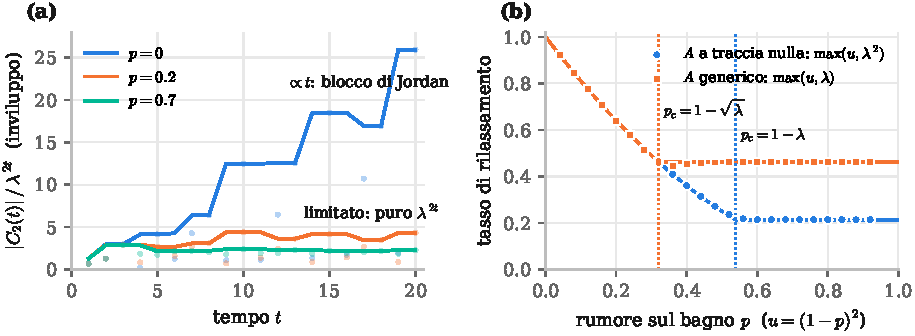
\includegraphics[width=\textwidth]{figs/fig_model2_rates.pdf}
\caption{Modello 2, OTOC a due repliche ($\lambda=0.462$). (a) OTOC compensato $|C_2(t)|/\lambda^{2t}$, con $A=B=Z$; si mostra l'inviluppo delle oscillazioni dovute agli autovalori complessi del canale. Senza rumore cresce linearmente in $t$ (blocco di Jordan); con rumore resta limitato. (b) Tasso di rilassamento asintotico in funzione di $p$. I punti sono la stima numerica su $t\in[14,24]$, le linee sono $\max(u,\lambda^2)$ e $\max(u,\lambda)$, e le verticali segnano gli incroci $p_c$.}
\label{fig:m2rates}
\end{figure}
\begin{figure}[t]
\centering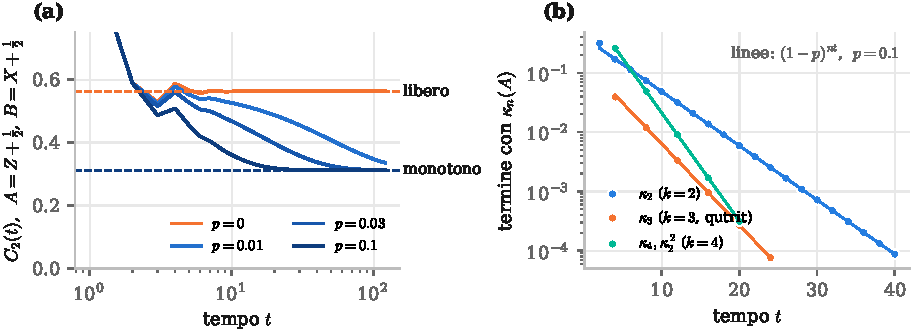
\includegraphics[width=\textwidth]{figs/fig_model2_free.pdf}
\caption{Modello 2, free probability e rumore. (a) $C_2(t)$ per $A=Z+\tfrac12$, $B=X+\tfrac12$: senza rumore tende al valore libero, con qualunque rumore al valore monotono $\varphi(A)^2\varphi(B^2)$. (b) Spettroscopia dei cumulanti a $p=0.1$: il termine proporzionale a $\kappa_n(A)$ decade come $(1-p)^{nt}$ (linee), per $n=2,3,4$.}
\label{fig:m2free}
\end{figure}
\subsection{Risultati}
I risultati sono riassunti nelle \cref{fig:m2rates,fig:m2free}.

\begin{proposition}[valori a tempi lunghi]\label{prop:mono}
Senza rumore, $C_k(\infty)=\sum_{\pi\in NC(k)}\kappa_\pi(A)\,\varphi_{K(\pi)}(B)$: $A(t)$ e $B$ sono liberi. Verificato per $k=2,3$, con qubit e qutrit.

Con qualunque rumore ($p>0$, su E, su C o su A) si ha invece
\[
C_k(\infty)=\varphi(A)^k\,\varphi(B^k).
\]
È la regola dell'indipendenza \emph{monotona} con $A(t)\succ B$. Equivale a dire che, in ogni momento a più repliche, $A(t)\to\varphi(A)\,\mathbb 1$.
\end{proposition}

\begin{proposition}[spettroscopia dei cumulanti liberi]\label{prop:spectro}
Con rumore sul bagno, il contributo a $C_k(t)$ proporzionale a $\kappa_n(A)$ decade come $(1-p)^{nt}$. Numericamente:
\begin{itemize}[leftmargin=1.5em]
\item $n=2$, $k=2$ e $k=3$, $p=0.1$: tasso $0.809$ contro $(0.9)^2=0.81$;
\item $n=3$, $k=3$ con qutrit, $p=0.1$: tasso $0.7290$ contro $(0.9)^3=0.729$.
\end{itemize}
Interpretazione: un cumulante libero di ordine $n$ richiede $n$ copie la cui eco sopravvive, e ogni copia sopravvive al rumore con probabilità $1-p$ per passo.
\end{proposition}

\noindent \emph{Meccanismo.} Il depolarizzante agisce su un'etichetta $\sigma\in S_k$ come
\[
\mathcal N^{\dagger\otimes k}(P_\sigma)=(1-p)^{\,k-\mathrm{fix}(\sigma)}\,P_\sigma+O(1/D),
\]
dove $\mathrm{fix}(\sigma)$ è il numero di punti fissi di $\sigma$. Infatti i sottoinsiemi di copie depolarizzate contenuti nei punti fissi riproducono $P_\sigma$, mentre togliere un punto mosso costa un fattore $1/D$.

Nella formula a multicatene, il termine $\kappa_\pi(A)\varphi_{K(\pi)}(B)$ resta a lungo sull'etichetta $\pi$. Ci aspettiamo quindi che decada come $(1-p)^{(k-\#\text{singoletti}(\pi))\,t}$. Verifica a $k=4$, con $A=Z$ a traccia nulla, $B=X+\tfrac12$ e $p=0.1$: i termini sopravvissuti, $\kappa_4(A)$ e $\kappa_2(A)^2$, spostano tutte e 4 le copie. Il tasso misurato è $0.6561=(1-p)^4$. Senza rumore si riproduce il valore libero $2b^2+b^4=0.5625$. Una dimostrazione per $k$ generico, sul reticolo $NC(k)$, è ancora da scrivere.

\begin{proposition}[incrocio netto dei tassi]\label{prop:cross}
Il rilassamento asintotico di $C_2(t)-C_2(\infty)$ ha tasso
\[
\max\bigl(u,\ \lambda^m\bigr),
\]
con $m=2$ per $A$ a traccia nulla e $m=1$ altrimenti. C'è quindi un incrocio netto in $p_c=1-\lambda^{m/2}$: per il gate di prova, $p_c=0.538$ con $m=2$ e $0.32$ con $m=1$. Vicino all'incrocio compare un prefattore lineare di tipo Jordan. Nelle tabelle in \cref{app:num2}, a $p=0.1$ il tasso misurato è $0.8100=u$, a $p=0.7$ è $0.2140\approx\lambda^2$.
\end{proposition}

\noindent \textbf{Risposta alla domanda Q7 delle note} (crossover o transizione al crescere del rumore). In questo modello il tasso asintotico ha un punto non analitico, quindi la transizione è netta. A tempi finiti è un crossover, con tempo caratteristico $\sim1/(2p)$.

\paragraph{Limiti.} A $D=\infty$ il rumore su una parte \emph{finita} del bagno è irrilevante, perché l'etichetta vive su tutto E. Per il rumore locale nel bagno serve $D$ finito: è esattamente la situazione del modello 1, dove l'incrocio dipende da $pL$. Resta da dimostrare analiticamente la legge $(1-p)^{nt}$ per $k$ generico, sul reticolo $NC(k)$.

\section{Esplorazione: un IPR per i process tensor}\label{sec:ipr}

\CartoonIPR
\subsection{Definizione}
La ``base'' di un process tensor è uno \emph{strumento}: a ogni passo si prepara e si misura il sistema in una certa base. Usiamo la misura proiettiva di S a ogni passo, con lo stato collassato che prosegue nella dinamica. Ne risulta una distribuzione dei record $p(x_1,\dots,x_n)$ su $N=d^n$ storie, con:
\begin{itemize}[leftmargin=1.5em]
\item \textbf{IPR temporale} $\mathcal I_2=\sum_xp(x)^2$, e il suo valore normalizzato $N\mathcal I_2$;
\item \textbf{valori di riferimento}: $N\mathcal I_2=1$ per record uniformi, $\simeq2$ per Porter--Thomas, crescita esponenziale in $n$ per una distribuzione moltiplicativa (log-normale);
\item \textbf{testimone di memoria}. Per un processo Markoviano (prodotto) e uno strumento prodotto con preparazioni fissate, $p$ si fattorizza e $\log\mathcal I_2$ è additivo. La non additività
\[
\Delta I_{\rm rec}=\log_2\frac{\mathcal I_2(\text{tutto})}{\mathcal I_2(\text{passato})\,\mathcal I_2(\text{futuro})}
\]
è quindi un testimone operativo di memoria.
\end{itemize}

\subsection{Risultati esatti nel modello 1}
Senza rumore, la matrice di trasferimento a due repliche per un passo registrato è simmetrica, con autovalori
\[
\lambda_\pm=\frac{D\pm1}{dD\pm1}
\]
sui sottospazi simmetrico e antisimmetrico di E$\otimes$E. Ne segue
\[
\mathcal I_2(n)=\tfrac{1+P_{\rm E}}{2}\,\lambda_+^n+\tfrac{1-P_{\rm E}}{2}\,\lambda_-^n ,
\]
verificato con il Monte Carlo per $D=2,3$, con ambiente puro o misto e con rumore (ricorsione generale), entro $1$--$2\sigma$. Per $D=1$ si ritrova il prodotto di fattori Porter--Thomas, $N\mathcal I_2=(2d/(d+1))^n$.

\begin{figure}[t]
\centering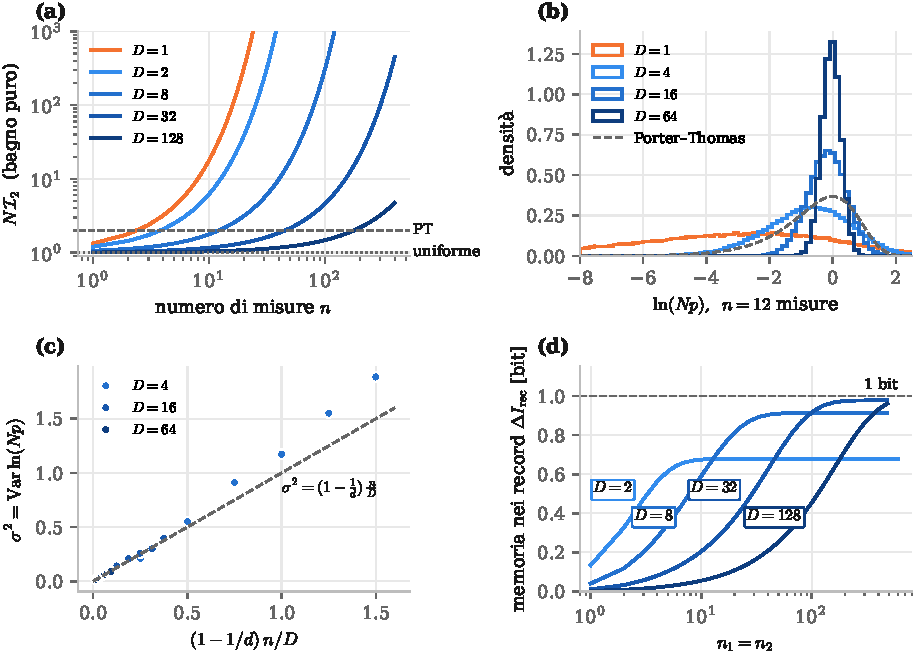
\includegraphics[width=\textwidth]{figs/fig_ipr.pdf}
\caption{IPR temporale nel modello 1 ($d=2$). (a) IPR normalizzato $N\mathcal I_2$ con bagno puro: 1 corrisponde a record uniformi, 2 a Porter--Thomas. Senza bagno ($D=1$) la crescita esponenziale è immediata; con un bagno grande i record restano quasi uniformi fino a $n\sim D$. (b) Istogrammi di $\ln(Np)$ a $n=12$ (Monte Carlo): sono log-normali e si stringono al crescere di $D$; tratteggiata la Porter--Thomas. (c) Collasso della varianza su $\sigma^2=(1-1/d)\,n/D$. (d) Memoria vista nei record, $\Delta I_{\rm rec}$: satura sotto 1 bit, mentre la memoria quantistica è $2\log_2D$, cioè 2, 6, 10 e 14 bit per $D=2,8,32,128$.}
\label{fig:ipr}
\end{figure}
\paragraph{La distribuzione temporale è log-normale (\cref{fig:cartoon-ipr,fig:ipr}).} Con il Monte Carlo sulle probabilità dei record (bagno puro, $d=2$):
\begin{itemize}[leftmargin=1.5em]
\item $\ln(Np)$ ha varianza $\sigma^2\simeq(1-\tfrac1d)\,n/D$ (pendenza misurata $0.58$, $0.52$, $0.51$ volte $1/D$ per $D=4,16,64$) e media $-\sigma^2/2$;
\item vale $N\mathcal I_2=e^{\sigma^2}=(d\lambda_+)^n$, e la media quenched coincide con quella annealed per $D\ge4$;
\item per $D=1$ la varianza cresce di circa $1.1$ per passo.
\end{itemize}
La distribuzione dei record è quindi \emph{moltiplicativa}, cioè ``Markoviana'' nel senso di prodotto di fattori. Non è mai Porter--Thomas. Il bagno rende i fattori quasi uniformi: i record restano quasi uniformi fino a
\[
n^*\simeq\ln2\,\frac{dD+1}{d-1}\qquad(N\mathcal I_2=2),
\]
dopodiché si allargano. La dimensione efficace del bagno si legge dal record di una sola sonda, tramite $\sigma^2/n=(1-1/d)/D$.

\paragraph{I record vedono poca memoria.} $\Delta I_{\rm rec}$ (annealed) satura a meno di 1 bit: $0.68$, $0.91$, $0.98$ bit per $D=2,8,32$, raggiunti su tempi $\sim D$. La memoria quantistica Rényi-2 è invece $2\log_2D$ (\cref{sec:model1}). Quasi tutta la memoria del process tensor è invisibile ai record in una base fissata. Il valore limite di 1 bit va verificato con medie quenched.

\paragraph{Bagno a temperatura infinita.} Con $P_{\rm E}=1/D$ le deviazioni dai record uniformi sono $O(n^2/D^2)$ invece che $O(n/D)$: a $n=4$, $N\mathcal I_2=1.039$ per $D=8$ misto contro $1.257$ per $D=8$ puro.

Questo è un caso di un fatto generale. Per un bagno scramblante grande a temperatura infinita, tutte le statistiche dei record ($\sum_xp^k$) coincidono con quelle del processo medio (una replica) a meno di correzioni $O(1/D^2)$. Il motivo è che i record legano le repliche solo sulle gambe di S, mentre E è tracciato replica per replica a entrambi i capi.

Lo stesso argomento dice che nel modello 2 a $D=\infty$ i record sono una catena di Markov classica, generata dal canale a una replica: tutta la fisica dell'eco è invisibile ai record.

\paragraph{Rumore.} Con rumore locale sull'ambiente sia la crescita di $N\mathcal I_2$ sia $\Delta I_{\rm rec}$ calano esponenzialmente in $L$. Per i record non abbiamo visto una transizione netta.

\subsection{La questione della base}
\begin{enumerate}[leftmargin=2em]
\item \textbf{Modelli Haar} (modello 1). La base è irrilevante per invarianza.
\item \textbf{Modelli strutturati} (collo di bottiglia, dual-unitari, Floquet). A $D$ grande la base entra solo tramite il canale a una replica. Le basi allineate ai modi lenti di $\mathcal M$ massimizzano le correlazioni temporali dei record.
\item \textbf{Versione indipendente dalla base.} Con preparazioni e misure in basi Haar indipendenti su ogni gamba, la media dell'IPR è
\[
\mathbb E_U\,\mathcal I_2=(d+1)^{-2n}\sum_{A\subseteq\text{gambe}}\operatorname{Tr}\Upsilon_A^2 .
\]
È l'analogo multi-tempo della formula delle misure randomizzate, e lega l'IPR temporale alle purezze dei marginali di $\Upsilon$, quindi a $I_2$.
\item \textbf{Base di operatori.} L'IPR della distribuzione di Pauli di $\Upsilon$, $\Xi(P)\propto\operatorname{Tr}(\Upsilon P)^2$, è un'entropia stabilizer del processo, cioè ``magia temporale''. È invariante per Clifford e naturale per WP-A; non l'abbiamo ancora calcolato.
\end{enumerate}

\subsection{Cosa ci sembra promettente}
\begin{itemize}[leftmargin=1.5em]
\item \textbf{Statistica log-normale dei record come sonda di bagni finiti.} Estrarre $D_{\rm eff}$ dalla crescita di $\sigma^2$ in modelli strutturati e in catene caotiche, a $D$ finito, dove i record vedono memoria.
\item \textbf{Test di Markovianità sui record.} Confrontare $p$ con la migliore catena di Markov, usando la mutua informazione condizionata di Shannon fra passato e futuro dato il presente. Va a zero a $D=\infty$ (modello 2); misurarne le correzioni $O(1/D)$.
\item \textbf{IPR di Pauli del process tensor.} È a quattro repliche ed è legato al doping.
\item \textbf{Record con eco.} Protocolli in cui i record legano le repliche anche dentro E, come le misure dell'ambiente o gli echi. Lì l'IPR temporale vede la fisica del settore $\circ$.
\end{itemize}

\section{Lavori correlati e cosa è nuovo}\label{sec:related}
Controllo di novità del 27 novembre 2026, fatto su abstract e testo HTML. Va ripetuto prima di scrivere un articolo: il campo si muove in fretta.

\paragraph{Modello 2.}
\begin{itemize}[leftmargin=1.5em]
\item \textbf{Il più vicino è \cite{GGW26}.} Studia OTOC di ordine $k$ in mappe caotiche. In assenza di rumore, i tassi dipendono solo dalla parità di $k$; con decoerenza diffusiva (coarse-graining nello spazio delle fasi), l'intero $k$-OTOC decade con tasso proporzionale a $k$. Il lavoro è numerico e non risolve i singoli cumulanti liberi.

  La nostra \cref{prop:spectro} è la versione esatta e risolta per cumulante: decade come $(1-p)^{nt}$ il termine con $\kappa_n(A)$, non l'OTOC intero, e il meccanismo è esplicito ($n$ copie con eco).
\item \textbf{\cite{YS25}} studia un'eco di Loschmidt per operatori, cioè una quantità a due repliche, con lo stesso rumore depolarizzante. Trova due regimi separati da un crossover graduale a $t\sim1/p$. Non ci sono OTOC di ordine $k$, né free probability, né incroci netti di tassi.
\item \textbf{\cite{SY23}}: nei sistemi aperti la dissipazione agisce in proporzione alla taglia dell'operatore. È un parente concettuale della spettroscopia dei cumulanti.
\item \textbf{\cite{VSHHLA25}}: bagno random risolto esattamente e transizione dell'entanglement temporale sotto coarse-graining delle misure, senza rumore.
\item \textbf{\cite{FGW25}}: cumulanti liberi in setup sistema--bagno chiusi.
\item \textbf{\cite{HB23}}: il rumore \emph{genera} la struttura libera (QSSEP). È la direzione opposta alla nostra, ma va citato.
\item Non abbiamo trovato lavori su indipendenza monotona in dinamica quantistica. Il nostro limite rumoroso è comunque banale ($A(t)\to\varphi(A)\mathbb 1$).
\item Gli incroci netti $\max(u,\lambda^m)$ e la rimozione del blocco di Jordan non compaiono nei lavori trovati.
\end{itemize}

\paragraph{Modello 1.}
\begin{itemize}[leftmargin=1.5em]
\item \textbf{Markovianizzazione per tipicità.} \cite{FMP19,FPM21} mostrano che i processi Haar sono quasi Markoviani a grande $D$. \cite{MRB23} trova che, in un modello di collisione, il backflow cala aumentando il numero di ancille, in modo graduale e senza rumore.

  Il nostro risultato è diverso. La memoria è non monotona in $L$ (cresce, poi crolla), c'è un incrocio netto con $L^*$ in forma chiusa, e un limite di scala in $x=pL$. Il meccanismo è analogo alla transizione indotta dal rumore nel random circuit sampling ($\varepsilon N\sim$ costante). Non l'abbiamo trovato per i process tensor.
\item \textbf{Spettro.} Che lo stato di Choi di un canale random segua Marchenko--Pastur è noto (misura indotta, \cite{IPR26} e riferimenti). L'estensione ai process tensor multi-tempo è naturale; è un risultato minore.
\item L'identità $\delta_{\rm HS}=1-2^{-I_2}$ per rumore unitale non l'abbiamo trovata, ma è un risultato piccolo.
\end{itemize}

\paragraph{Conclusione operativa.} Il pezzo più forte e più nuovo è la spettroscopia dei cumulanti con l'incrocio dei tassi (modello 2). Va presentata come versione esatta e risolta per cumulante di \cite{GGW26}, e conviene muoversi in fretta: i gruppi di Claeys, Lerose--Abanin e Wisniacki lavorano su temi adiacenti. La Markovianizzazione indotta dal rumore (modello 1) è un secondo lavoro naturale.

\section{Prossimi passi}\label{sec:next}
\begin{enumerate}[label=\textbf{N\arabic*.},leftmargin=2.2em]
\item \textbf{Legge generale dei cumulanti.} Dimostrare sul reticolo $NC(k)$ che il termine $\kappa_\pi(A)\varphi_{K(\pi)}(B)$ decade come $(1-p)^{(k-\#\text{singoletti}(\pi))t}$. Il meccanismo all'ordine dominante in $1/D$ è già nella \cref{sec:bottleneck}.
\item \textbf{Esperimenti.} In un esperimento di eco con rumore regolabile, i tassi $(1-p)^{n}$ separano i cumulanti liberi. L'idea è usare la decoerenza come spettroscopia della struttura libera dell'OTOC; i dati di eco dei processori superconduttori sono il banco di prova naturale.
\item \textbf{Rumore locale nel bagno a $D$ finito.} Collegare i due modelli: un bagno a collo di bottiglia con $L$ qudit rumorosi dovrebbe mostrare l'incrocio del modello 1, controllato da $pL$.
\item \textbf{Tempo continuo.} Un bagno Browniano dà il generatore esatto a $k$ repliche (domanda Q3 delle note), e permette di verificare l'inferenza che $\mathcal K$ sia di ordine $dt$.
\item \textbf{Quenched contro annealed.} Stabilire se gli incroci sopravvivono nelle quantità tipiche (limite di repliche $k\to1$), come nei lavori su RMPS.
\item \textbf{Randomness strutturata e doping.} Ripetere con bagni Clifford random (commutante di Clifford) e Gaussiani fermionici, poi con doping $T$ o non Gaussiano.
\end{enumerate}

\appendix
\section{Verifiche numeriche: modello 1}\label{app:num1}

Ogni formula della \cref{sec:model1} è verificata entro $2\sigma$ contro un Monte Carlo esatto, cioè la costruzione del process tensor completo a taglie piccole. Le verifiche includono un caso di rumore non unitale. Per $k\ge3$ a grande $D$ si usa aritmetica razionale esatta, perché la versione in virgola mobile del trasferimento su $S_k$ perde precisione.

\paragraph{Purezza} ($d=2$, $\rho_{\rm E}(0)=I/D$). Monte Carlo contro formula esatta: per $D=2$, $n=1,2,3$, si ha $0.4001(19)$, $0.2802(7)$, $0.2553(3)$ contro $0.4000$, $0.2800$, $0.2560$. Con depolarizzante globale $p=0.3$: $0.2186(9)$ e $0.1329(7)$ contro $0.2188$ e $0.1341$.

\paragraph{Posizione dell'incrocio} (esatto contro previsione $L^*\simeq\ln d^2/\ln(q^2/g_F)$).
\begin{center}\small
\begin{tabular}{@{}lcc@{}}
\toprule
canale & $L^*$ esatto & $L^*$ previsto\\
\midrule
depolarizzante, $p=0.1$ & 9.01 & 9.02\\
dephasing, $p=0.25$ & 2.94 & 2.95\\
amplitude damping, $\gamma=0.3$ & 4.70 & 4.71\\
\bottomrule
\end{tabular}
\end{center}

\paragraph{Limite di scala} (depolarizzante, $d=q=2$, $x^*=0.924$). Il rapporto $I_2^\infty/(2\log_2D)$ a $x=0.90$ vale $0.092$, $0.798$, $0.936$, $0.969$ per $p=0.1$, $0.03$, $0.01$, $0.005$. A $x=0.95$ vale $0$ per tutti i $p$.

\paragraph{Quenched contro annealed} ($d=q=2$, $n_1=n_2=8$).
\begin{center}\small
\begin{tabular}{@{}cccc@{}}
\toprule
$p$ & $I_2$ annealed ($L=1/2/3$) & $\langle I_2\rangle$ quenched & deviazione standard\\
\midrule
0.30 & 0.976 / 1.267 / 0.471 & 0.978 / 1.269 / 0.472 & 0.12 / 0.05 / 0.01\\
0.42 & 0.611 / 0.425 / 0.059 & 0.636 / 0.430 / 0.059 & 0.12 / 0.04 / 0.003\\
0.55 & 0.316 / 0.121 / 0.014 & 0.339 / 0.123 / 0.014 & 0.09 / 0.02 / 0.002\\
\bottomrule
\end{tabular}
\end{center}
L'informazione mutua di von Neumann ($n_1=n_2=2$, $\Upsilon$ completo) vale $0.90$ e $0.70$ bit per $L=1,2$ a $p=0.2$, e $0.40$ e $0.16$ a $p=0.42$.

\paragraph{Distanza dalla Markovianità.} L'identità a tre e quattro repliche è verificata in aritmetica razionale. Fallisce per amplitude damping: con $D=2$, $n_1=2$, $n_2=1$, $\gamma=0.5$ si ha $0.10517\neq0.10453$, confermato con il Monte Carlo. A grande $D$, per $n_1=n_2=1$ e $D=256$, $\delta_{\rm HS}D^2/d^{2n}=0.5624$ contro $0.5625$ previsto. La distanza di traccia vale $0.312$, $0.158$, $0.0795$ per $D=4$, $8$, $16$. Con rumore ($p=0.3$, $n_1=n_2=6$), per $L=1,\dots,5$: $\delta_{\rm HS}=0.49$, $0.57$, $0.25$, $0.023$, $0.0018$.

\paragraph{Spettro} (punto critico $c=N/M=1$, rapporto con la free Poisson per $k=2,3,4$): $0.992$, $0.982$, $0.970$ a $D=16$; $0.9993$, $0.9984$, $0.9974$ a $D=64$; $0.99995$, $0.99987$, $0.99980$ a $D=256$. A $n=8$ il rapporto è $1.000$.

\section{Verifiche numeriche: modello 2}\label{app:num2}

Gate di prova $U=(r_1\otimes r_2)\,e^{-i\tau(XX+YY+JZZ)}(r_2^\dagger\otimes r_1)$, con $\tau=0.5$, $J=0.3$ e rotazioni a un qubit fissate. L'autovalore subdominante del canale a una replica è $\lambda=0.4622$. Per i qutrit si usa un gate fisso casuale, con $\lambda=0.394$.

\paragraph{Ricorsione esatta contro Monte Carlo} (media su $V_s$ Haar; $A=B=Z$ per $k=2$, $A=Z+\tfrac12$, $B=X+\tfrac12$ per $k=3$).
\begin{center}\small
\begin{tabular}{@{}lccc@{}}
\toprule
caso & $t$ & Monte Carlo & esatto\\
\midrule
$k=2$, $D=2$, $p=0$ & 2 / 3 & $-0.0788(32)$ / $-0.0526(49)$ & $-0.0825$ / $-0.0483$\\
$k=2$, $D=3$, $p=0$ & 2 / 3 & $-0.0689(21)$ / $-0.0355(31)$ & $-0.0689$ / $-0.0373$\\
$k=2$, $D=2$, rumore su E $p=0.3$ & 3 & $-0.0460(30)$ & $-0.0452$\\
$k=2$, $D=2$, rumore su C $p=0.3$ & 3 & $-0.0260(17)$ & $-0.0247$\\
$k=3$, $D=2$, $p=0$ & 2 / 3 & $1.0828(93)$ / $1.0390(90)$ & $1.0865$ / $1.0310$\\
$k=3$, $D=2$ / $3$, $p=0.4$ & 3 & $0.6394(51)$ / $0.5993(30)$ & $0.6450$ / $0.5960$\\
\bottomrule
\end{tabular}
\end{center}
Il limite a due settori coincide con la ricorsione esatta a $D=10^3$ e $10^5$, a 6 cifre (per esempio $C_2(5)=-0.001840$ senza rumore e $-0.001189$ con $p=0.2$). Il codice generale in $k$ riproduce quello dedicato a $k=2$.

\paragraph{Valori a tempi lunghi} ($t=60$, $A=Z+a$, $B=X+b$, $k=2$). Valore libero $a^2+b^2+a^2b^2$, valore monotono $a^2(1+b^2)$.
\begin{center}\small
\begin{tabular}{@{}ccccccc@{}}
\toprule
$(a,b)$ & $p=0$ & $0.02$ & $0.1$ & $0.3$ & libero & monotono\\
\midrule
$(0.5,0)$ & 0.2500 & 0.2500 & 0.2500 & 0.2500 & 0.2500 & 0.2500\\
$(0,0.5)$ & 0.2500 & 0.0242 & 0.0000 & 0.0000 & 0.2500 & 0\\
$(0.5,0.7)$ & 0.8625 & 0.4199 & 0.3725 & 0.3725 & 0.8625 & 0.3725\\
$(1,1)$ & 3.0000 & 2.0967 & 2.0000 & 2.0000 & 3.0000 & 2.0000\\
\bottomrule
\end{tabular}
\end{center}
Con rumore su C ($p=0.3$ e $0.8$) o su A ($p=0.3$) si ottiene lo stesso valore monotono, $0.3125$ per $(a,b)=(0.5,0.5)$.

A $k=3$ (qubit, $a=b=\tfrac12$): valore libero $1.140625$, monotono $0.203125$. Si trova $1.140625$ senza rumore. Con $p=0.1$ il valore tende a $0.2031$ con tasso $0.809\approx(1-p)^2$; con $p=0.3$, a $t=40$, si ha $0.203125$. Con i qutrit, $A=\mathrm{diag}(1,1,-2)$ e $B=\mathrm{diag}(1,0,0)$: il valore libero $\kappa_3(A)\varphi(B)^3=-0.074074$ è riprodotto senza rumore, e con $p=0.1$ il segnale decade con tasso $0.7290=(1-p)^3$. A $k=4$ (qubit, $A=Z$, $B=X+\tfrac12$): $C_4(14)=C_4(20)=0.562500$ senza rumore, che è il valore libero $2b^2+b^4$. Con $p=0.1$ il tasso è $0.6561=(1-p)^4$.

\paragraph{Tassi di rilassamento} ($k=2$, $A=Z$, $B=X+\tfrac12$, tasso stimato su $t\in[14,24]$).
\begin{center}\small
\begin{tabular}{@{}lccccccc@{}}
\toprule
$p$ & 0.1 & 0.3 & 0.45 & 0.5 & 0.55 & 0.6 & 0.7\\
\midrule
tasso & 0.8100 & 0.4900 & 0.3028 & 0.2525 & 0.2207 & 0.2142 & 0.2140\\
$\max(u,\lambda^2)$ & 0.8100 & 0.4900 & 0.3025 & 0.2500 & 0.2136 & 0.2136 & 0.2136\\
\bottomrule
\end{tabular}
\end{center}
Per $A=Z+\tfrac12$ il tasso misurato è invece $\max(u,\lambda)$: $0.4866$ a $p=0.3$ ($u=0.49$), e $0.459$--$0.460$ per $p\ge0.45$ ($\lambda=0.462$).

\begin{thebibliography}{99}\small
\bibitem{FC25} F.~Fritzsch, P.~W.~Claeys, \emph{Free probability in a minimal quantum circuit model}, Phys.\ Rev.\ X \textbf{16}, 031027 (2026), arXiv:2506.11197.
\bibitem{FARC25} F.~Fritzsch, G.~O.~Alves, M.~A.~Rampp, P.~W.~Claeys, \emph{Free cumulants and full eigenstate thermalization from boundary scrambling}, PRX Quantum \textbf{7}, 043003 (2026), arXiv:2509.08060.
\bibitem{DDHTP25} N.~Dowling, J.~De Nardis, M.~Heinrich, X.~Turkeshi, S.~Pappalardi, \emph{Free independence and unitary design from random matrix product unitaries}, arXiv:2508.00051 (2025).
\bibitem{LDT25} G.~Lami, J.~De Nardis, X.~Turkeshi, \emph{Anticoncentration and state design of random tensor networks}, Phys.\ Rev.\ Lett.\ \textbf{134}, 010401 (2025).
\bibitem{LDTD25} G.~Lami, A.~De Luca, X.~Turkeshi, J.~De Nardis, \emph{Quantum state design and emergent confinement mechanism in measured tensor network states}, arXiv:2504.16995 (2025).
\bibitem{FMP19} P.~Figueroa-Romero, K.~Modi, F.~A.~Pollock, \emph{Almost Markovian processes from closed dynamics}, Quantum \textbf{3}, 136 (2019), arXiv:1802.10344.
\bibitem{FPM21} P.~Figueroa-Romero, F.~A.~Pollock, K.~Modi, \emph{Markovianization with approximate unitary designs}, Commun.\ Phys.\ \textbf{4}, 127 (2021), arXiv:2004.07620.
\bibitem{TS24} X.~Turkeshi, P.~Sierant, \emph{Error-resilience phase transitions in encoding-decoding quantum circuits}, Phys.\ Rev.\ Lett.\ \textbf{132}, 140401 (2024).
\bibitem{Mur01} N.~Muraki, \emph{Monotonic independence, monotonic central limit theorem and monotonic law of small numbers}, Infin.\ Dimens.\ Anal.\ Quantum Probab.\ Relat.\ Top.\ \textbf{4}, 39 (2001).
\bibitem{NS06} A.~Nica, R.~Speicher, \emph{Lectures on the Combinatorics of Free Probability}, Cambridge University Press (2006).
\bibitem{GGW26} N.~Gómez Brucks, I.~García-Mata, D.~A.~Wisniacki, \emph{Higher order OTOCs in chaotic quantum maps: Ruelle--Pollicott resonances and asymptotic freeness}, arXiv:2610.34615 (2026).
\bibitem{YS25} T.~Yoshimura, L.~Sá, \emph{Dynamics of Loschmidt echoes from operator growth}, Phys.\ Rev.\ B \textbf{113}, 144306 (2026), arXiv:2509.01585.
\bibitem{SY23} T.~Schuster, N.~Y.~Yao, \emph{Operator growth in open quantum systems}, Phys.\ Rev.\ Lett.\ \textbf{131}, 160402 (2023), arXiv:2208.12272.
\bibitem{VSHHLA25} I.~Vilkoviskiy, M.~Sonner, Q.~C.~Huang, W.~W.~Ho, A.~Lerose, D.~A.~Abanin, \emph{Temporal entanglement transition in chaotic quantum many-body dynamics}, PRX Quantum (2026), arXiv:2511.03846.
\bibitem{FGW25} M.~Füllgraf, J.~Gemmer, J.~Wang, \emph{Scaling of free cumulants in closed system-bath setups}, SciPost Phys.\ Core \textbf{9}, 025 (2026), arXiv:2511.11333.
\bibitem{HB23} L.~Hruza, D.~Bernard, \emph{Coherent fluctuations in noisy mesoscopic systems, the open quantum SSEP and free probability}, Phys.\ Rev.\ X \textbf{13}, 011045 (2023), arXiv:2204.11680.
\bibitem{MRB23} W.~F.~Magalhães, C.~O.~A.~Ribeiro Neto, B.~de Lima Bernardo, \emph{Unveiling the Markovian to non-Markovian transition with quantum collision models}, Physics Open \textbf{15}, 100144 (2023), arXiv:2210.11976.
\bibitem{IPR26} \emph{Probabilistic and approximate universal quantum purification machines}, arXiv:2604.06325 (2026) (sezione sui canali random e Marchenko--Pastur).
\end{thebibliography}

\end{document}
